\chapter{Comparaci�n}

Dado que los tres modelos analizados utilizan datos a un nivel de agregaci�n diferente, en ventanas de tiempo distintas, no resulta conveniente comparar los modelos frente al ajuste de  los periodos que se usaron como base para la estimaci�n. La comparaci�n se realiza entonces comparando las proyecciones realizadas, con las mediciones reales de poblaci�n en un periodo de validaci�n. El periodo de validaci�n considerado es desde enero de 2017 hasta mayo de 2018.

Para realizar la comparaci�n se debieron realizar ajustes en las proyecciones de raz�n-censal y estado-espacio. En el caso de la raz�n-censal se utiliz� suavizamiento a trav�s de una serie de tiempo estructural, para llevar la proyecci�n anual a nivel mensual. En las proyecciones por modelos estado-espacio se realiz� un ajuste en el orden de magnitud de las proyecciones, puesto que las proyecciones de delitos no son iguales a la poblaci�n total; se calcul� un factor de ajuste como la raz�n entre la poblaci�n total observada y la suma de poblaciones por delito. Las proyecciones ajustadas se observan en la tabla \ref{tab:Pronosticos} y la gr�fica \ref{fig:modelos}. El error de pron�stico definido como $proyectado - real$ se presenta en la tabla \ref{tab:Errorpronostico}

\begin{figure}[ht]
	\centering
	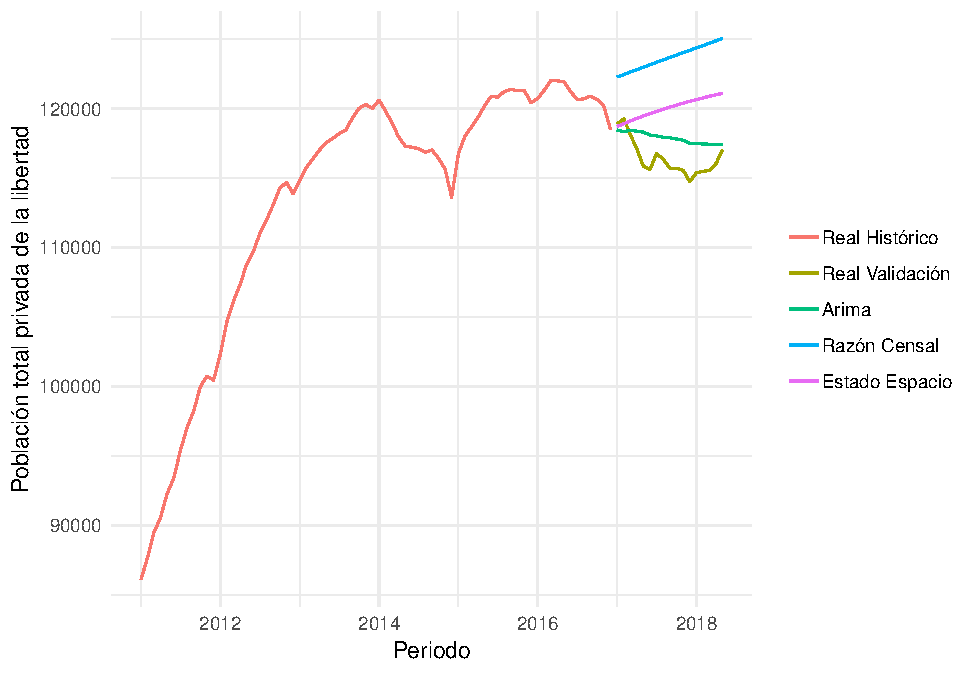
\includegraphics[width=10cm]{pry_compara-1.pdf}
	\caption{Proyecciones de Poblaci�n privada de la libertad Enero 2017 - Mayo 2018} {Fuente: INPEC} {Elaboraci�n propia}
	\label{fig:modelos}
\end{figure}

% latex table generated in R 3.5.1 by xtable 1.8-3 package
% Tue Nov 13 03:48:30 2018
\begin{table}[H]
	\centering
	\begin{tabular}{rlrrrr}
		\hline
		& Periodo & Real Validaci�n & Arima & Raz�n Censal & Estado Espacio \\ 
		\hline
		1 & 2017-01-01 & 118925 & 118466 & 122299 & 118733 \\ 
		2 & 2017-02-01 & 119269 & 118354 & 122466 & 118928 \\ 
		3 & 2017-03-01 & 118186 & 118446 & 122638 & 119116 \\ 
		4 & 2017-04-01 & 117119 & 118392 & 122814 & 119299 \\ 
		5 & 2017-05-01 & 115878 & 118315 & 122992 & 119475 \\ 
		6 & 2017-06-01 & 115628 & 118111 & 123171 & 119646 \\ 
		7 & 2017-07-01 & 116773 & 118045 & 123348 & 119810 \\ 
		8 & 2017-08-01 & 116373 & 117953 & 123523 & 119968 \\ 
		9 & 2017-09-01 & 115708 & 117909 & 123698 & 120120 \\ 
		10 & 2017-10-01 & 115721 & 117825 & 123872 & 120265 \\ 
		11 & 2017-11-01 & 115562 & 117738 & 124045 & 120405 \\ 
		12 & 2017-12-01 & 114750 & 117508 & 124216 & 120538 \\ 
		13 & 2018-01-01 & 115396 & 117488 & 124388 & 120666 \\ 
		14 & 2018-02-01 & 115488 & 117463 & 124558 & 120787 \\ 
		15 & 2018-03-01 & 115563 & 117451 & 124728 & 120901 \\ 
		16 & 2018-04-01 & 116058 & 117440 & 124897 & 121010 \\ 
		17 & 2018-05-01 & 117026 & 117431 & 125066 & 121112 \\ 
		\hline
	\end{tabular}
	\caption{Proyecciones y observado enero 2017 a mayo 2018} 
	\label{tab:Pronosticos}
\end{table}

% latex table generated in R 3.5.1 by xtable 1.8-3 package
% Tue Nov 13 03:49:20 2018
\begin{table}[H]
	\centering
	\begin{tabular}{rlrrr}
		\hline
		& Periodo & Arima & Raz�n Censal & Estado Espacio \\ 
		\hline
		1 & 2017-01-01 & -459 & 3374 & -192 \\ 
		2 & 2017-02-01 & -915 & 3197 & -341 \\ 
		3 & 2017-03-01 & 260 & 4452 & 930 \\ 
		4 & 2017-04-01 & 1273 & 5695 & 2180 \\ 
		5 & 2017-05-01 & 2437 & 7114 & 3597 \\ 
		6 & 2017-06-01 & 2483 & 7543 & 4018 \\ 
		7 & 2017-07-01 & 1272 & 6575 & 3037 \\ 
		8 & 2017-08-01 & 1580 & 7150 & 3595 \\ 
		9 & 2017-09-01 & 2201 & 7990 & 4412 \\ 
		10 & 2017-10-01 & 2104 & 8151 & 4544 \\ 
		11 & 2017-11-01 & 2176 & 8483 & 4843 \\ 
		12 & 2017-12-01 & 2758 & 9466 & 5788 \\ 
		13 & 2018-01-01 & 2092 & 8992 & 5270 \\ 
		14 & 2018-02-01 & 1975 & 9070 & 5299 \\ 
		15 & 2018-03-01 & 1888 & 9165 & 5338 \\ 
		16 & 2018-04-01 & 1382 & 8839 & 4952 \\ 
		17 & 2018-05-01 & 405 & 8040 & 4086 \\ 
		\hline
	\end{tabular}
	\caption{Error de pron�stico enero 2017 a mayo 2018} 
	\label{tab:Errorpronostico}
\end{table}

% latex table generated in R 3.5.1 by xtable 1.8-3 package
% Tue Nov 13 03:49:59 2018
\begin{table}[H]
	\centering
	\begin{tabular}{rr}
		\hline
		& Sesgo \\ 
		\hline
		Arima & 1465 \\ 
		Raz�n Censal & 7253 \\ 
		Estado Espacio & 3609 \\ 
		\hline
	\end{tabular}
	\caption{Sesgo de pron�stico enero 2017 a mayo 2018} 
	\label{tab:Sesgo}
\end{table}

El modelo ARIMA que considera la suma de la poblaci�n sindicada y la condenada es el que presenta el mejor desempe�o. Este tipo de modelos presentan un desempe�o adecuado en el corto plazo; sin embargo, al ser series integradas los intervalos de confianza del pron�stico divergen aceleradamente, haci�ndolo menos apropiado para proyecciones de largo plazo.

Tanto el forecast de los los modelos estado espacio como el modelo de poblaciones peque�as sobre-estiman el crecimiento de la poblaci�n carcelaria. Este escenario puede ser coyuntural, si se considera que la poblaci�n carcelaria decreci� durante 2016. Dado que el sesgo de ambos modelos era mayor al de los modelos SARIMA no se utilizan otros criterios de comparaci�n como el error absoluto medio.
